\documentclass[onecolumn]{article}
\usepackage{url}
\usepackage{algorithmic}
\usepackage[a4paper]{geometry}
\usepackage{datetime}
\usepackage[margin=2em, font=small,labelfont=it]{caption}
\usepackage{graphicx}
\usepackage{mathpazo} % use palatino
\usepackage[scaled]{helvet} % helvetica
\usepackage{microtype}
\usepackage{amsmath}
\usepackage{subfigure}
% Letterspacing macros
\newcommand{\spacecaps}[1]{\textls[200]{\MakeUppercase{#1}}}
\newcommand{\spacesc}[1]{\textls[50]{\textsc{\MakeLowercase{#1}}}}

\title{\spacecaps{Lab report: SW01 }\\ \normalsize \spacesc{TSM\_AnTeDe} }

\author{Fabian Gröger\thanks{fabian.groeger@hslu.ch}\\Hochschule Luzern}
\date{\today}

\begin{document}
\maketitle

\section{Lab 1a: Setting up the environment}
This notebook was only used as installation instruction and thus is not further discussed.

\section{Lab 1b: Text segmentation with nltk}
In this notebook we started off by downloading a book from the Gutenberg Project. This text was then used throughout the exercise. First the goal was to trim the text by removing the leading and trailing text, which corresponds to the intro and the license of the book. Afterwards the text was segmented into sentences and line-by-line written into a text file. This showed that overall \verb|nltk| did a great job on detecting the sentences. However, there were still some sentences, that were wrongly segmented. Most of them were either small sentence fragments, e.g. "just so." or were in direct speach. Then the sentences were tokenized and again saved in a file. This showed that the tokenization worked good and didn't show any unexpected results.

Using \verb|nltk.Text| an object was created from the word tokens which enabled us to apply some auxiliary function to the text, such as \verb|concordance|, \verb|similar| and \verb|collocations|. The \verb|concordance| showed exact matches of the given word, where as the \verb|similar| displayed sentences that contained words similar to the given one. And the \verb|collocation| showed words that often appear together, which showed, that most of these collocations are names in the text.

\begin{figure}[t]
\centering
    
\includegraphics[width=.3\linewidth]{fig/flat.png}
\caption{\label{fig:demo-bad}
Caption}
\end{figure}

\begin{figure}[t]
\centering
\subfigure[Standard rendering]{\centering
    
\includegraphics[width=.3\linewidth]{fig/flat.png}
        \label{fig:demo-standard}}
\subfigure[Fancy rendering]{\centering
    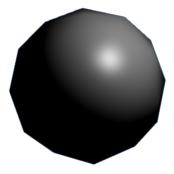
\includegraphics[width=.3\linewidth]{fig/smooth.png}
        \label{fig:demo-fancy}}
\caption{\label{fig:demo} 
Caption}
\end{figure}

\end{document}

